\documentclass{article}

\usepackage{tikz}

%--------------------------------------------------
%: math3d
\tikzset{math3d/.style={x={(-0.353cm,-0.353cm)},z={(0cm,1cm)},y={(1cm,0cm)}}}

%--------------------------------------------------
\begin{document}

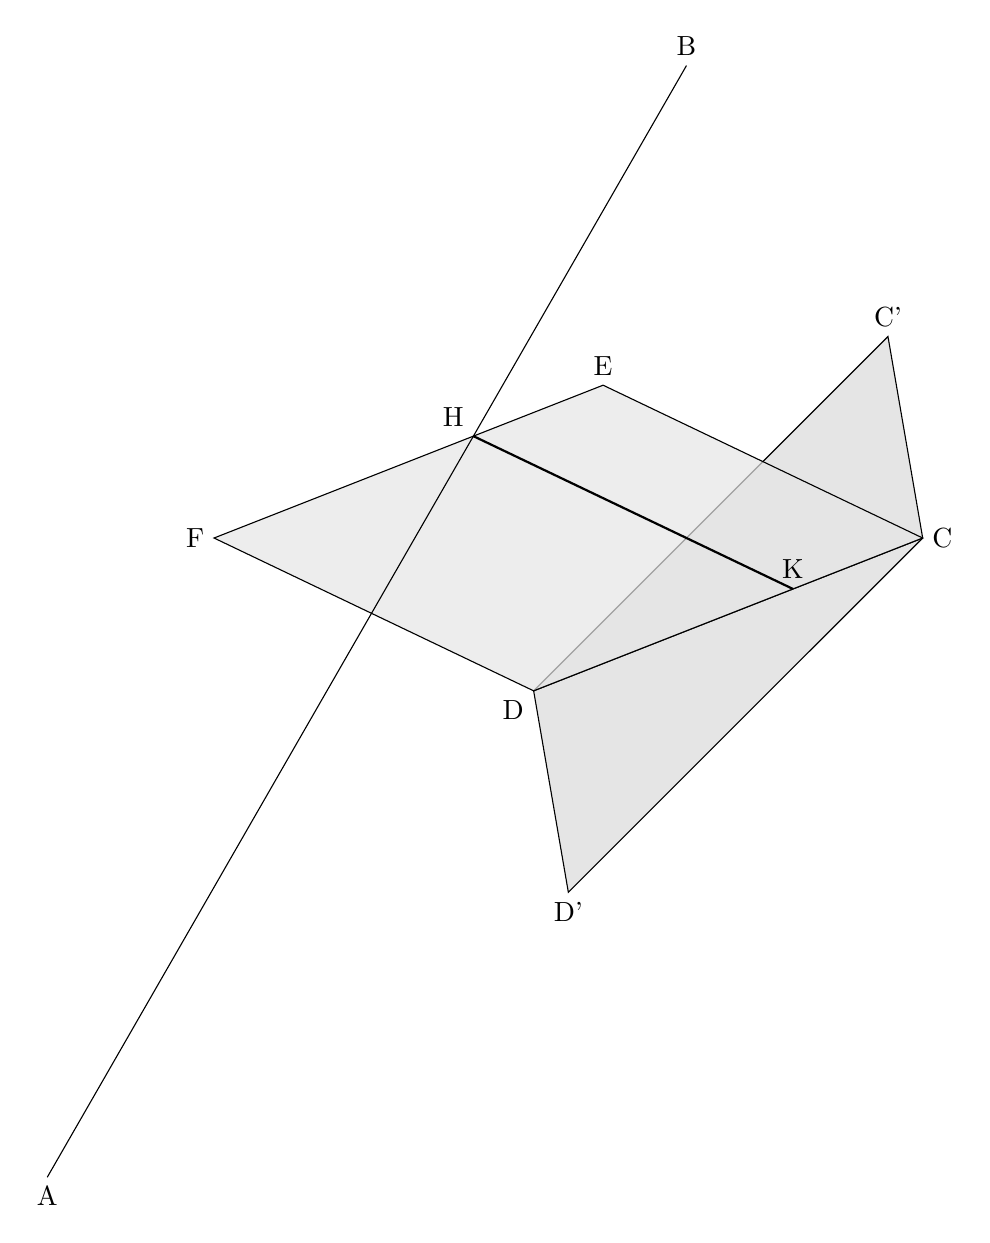
\begin{tikzpicture}[math3d,scale=3]
	\coordinate (a) at (2,-1,-2);
	\coordinate (b) at (0,1,2);
	\coordinate (c) at (0,2,0);
	\coordinate (d) at (-1,0,-1);
	\coordinate (h) at (2/3,1/3,2/3);
	\coordinate (k) at (-1/3,4/3,-1/3);
	\coordinate (c1) at (1,3/2,3/2);
	\coordinate (d1) at (0,-1/2,1/2);
	\coordinate (b1) at (-1,3/2,1/2);
	\coordinate (a1) at (0,1/2,-3/2);
	\coordinate (e) at (1,1,1);
	\coordinate (f) at (0,-1,0);
	\filldraw[fill=gray!20] (a1) node[below] {D'}
	    -- (c) -- (b1) node[above]{C'} -- (d) -- cycle;
	\draw (c) node[right]{C}-- (d) node[below left]{D};
	\draw (h) node[above left] {H};
	\fill[fill=gray!20,opacity=0.7] (c) -- (1,1,1) -- (0,-1,0) -- (d) -- cycle;
	\draw (c) --  (e) node[above]{E}-- (f)node[left]{F} -- (d) -- cycle ;
	\draw (a) node[below]{A}-- (b) node[above] {B};
	\draw [thick] (h)  -- (k) node[above]{K};
\end{tikzpicture}

\end{document}
